\documentclass{standalone}

\usepackage{tikz}
\usetikzlibrary{calc,patterns,arrows,shapes.arrows,intersections}
\usetikzlibrary{decorations,babel}
\usepackage{wasysym}
\usepackage{siunitx}
\usepackage[simplified]{pgf-umlcd}

\newlength\thickness
\pgfdeclarepatternformonly[\thickness]{section}
{\pgfpointorigin}
{\pgfpoint{0.5cm}{0.5cm}}
{\pgfpoint{0.5cm}{0.5cm}}
{
\pgfsetstrokecolor{black!50}
\pgfsetlinewidth{\thickness}
\pgfpathmoveto{\pgfpoint{0cm}{0cm}}
\pgfpathlineto{\pgfpoint{0.125cm}{0.125cm}}
\pgfpathclose
\pgfsetlinewidth{\thickness}
\pgfpathmoveto{\pgfpoint{0.125cm}{0cm}}
\pgfpathlineto{\pgfpoint{0cm}{0.125cm}}
\pgfpathclose
\pgfsetlinewidth{\thickness}
\pgfpathmoveto{\pgfpoint{0.25cm}{0.25cm}}
\pgfpathlineto{\pgfpoint{0.375cm}{0.375cm}}
\pgfpathclose
\pgfsetlinewidth{\thickness}
\pgfpathmoveto{\pgfpoint{0.25cm}{0.375cm}}
\pgfpathlineto{\pgfpoint{0.375cm}{0.25cm}}
\pgfpathclose
\pgfsetlinewidth{\thickness}
\pgfpathmoveto{\pgfpoint{0cm}{0.25cm}}
\pgfpathlineto{\pgfpoint{0.125cm}{0.375cm}}
\pgfpathclose
\pgfsetlinewidth{\thickness}
\pgfpathmoveto{\pgfpoint{0cm}{.375cm}}
\pgfpathlineto{\pgfpoint{.125cm}{0.25cm}}
\pgfpathclose
\pgfsetlinewidth{\thickness}
\pgfpathmoveto{\pgfpoint{0.375cm}{0.125cm}}
\pgfpathlineto{\pgfpoint{0.25cm}{0cm}}
\pgfpathclose
\pgfsetlinewidth{\thickness}
\pgfpathmoveto{\pgfpoint{0.375cm}{0cm}}
\pgfpathlineto{\pgfpoint{0.25cm}{0.125cm}}
\pgfusepath{stroke}
}

\tikzset{
thickness/.store in = \thickness,
thickness           = 0.5pt
}

\renewcommand{\aggregation}[4]{
\draw[umlcd style, -open diamond] (#1) -- (#4)
node[near end, above]{#2}
node[near end, below]{#3};
}

\renewcommand{\composition}[4]{
\draw[umlcd style, fill=\umldrawcolor, -diamond] (#1) -- (#4)
node[near end, above]{#2}
node[near end, below]{#3};
}

\begin{document}

\author{Luis Fernando Umaña}
\title{Diagrama de clases: Base de datos FRX}

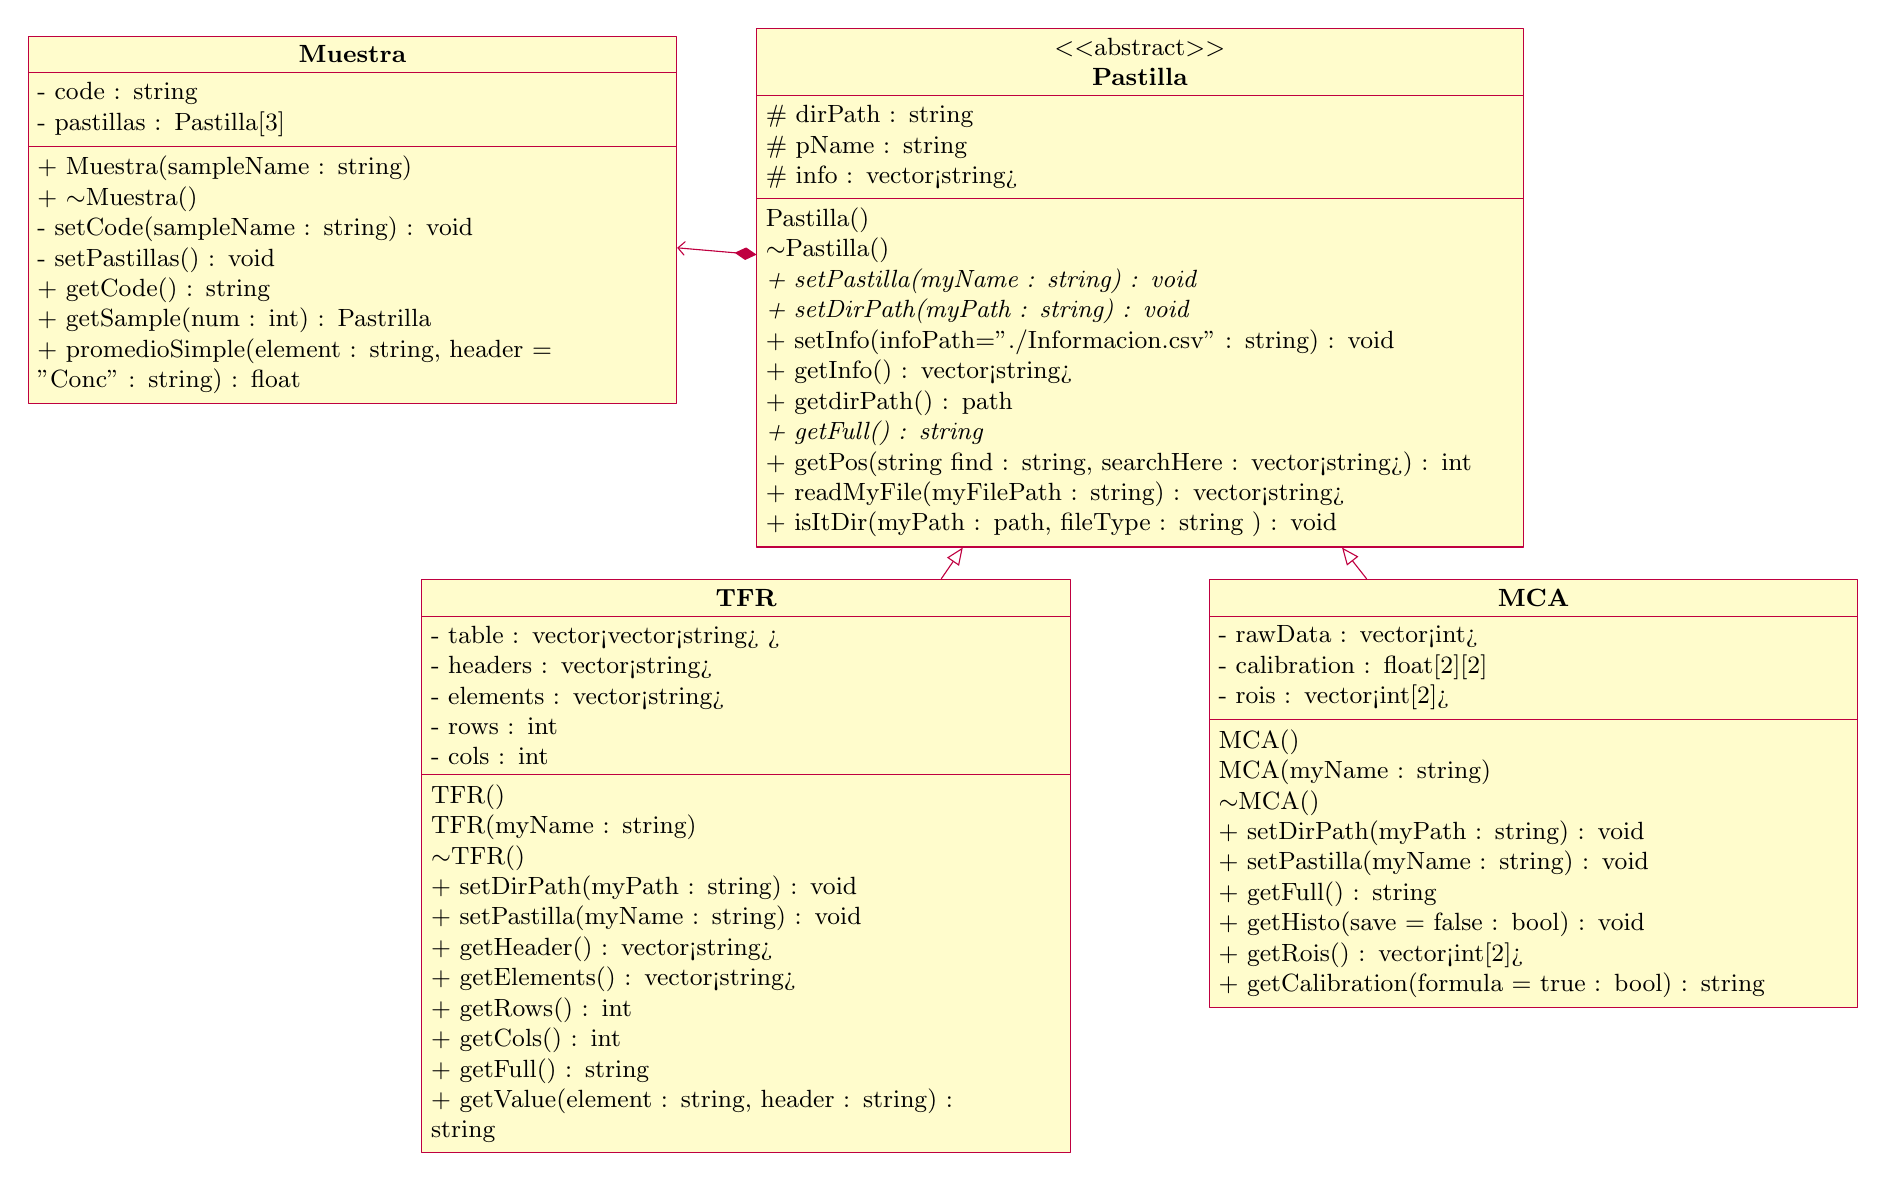
\begin{tikzpicture}[x         = 1cm,
                    y         = 1cm,
                    >         = latex,
                    line join = round,
                    font      = \small]

%-> Origin definition
%\coordinate (o) at (0,0);
	\begin{class}[text width = 8 cm]{Muestra}{0,-0.1}
		\attribute{- code : string}
		\attribute {- pastillas : Pastilla[3]}
		%-------------------------------------------------%
		\operation{+ Muestra(sampleName : string)}
		\operation{+ $\sim$Muestra()}
		\operation{- setCode(sampleName : string) : void}
		\operation{- setPastillas() : void}
		\operation{+ getCode() : string}
		\operation{+ getSample(num : int) : Pastrilla}
		\operation{+ promedioSimple(element : string, header = "Conc" : string) : float}
	\end{class}
	
	\begin{abstractclass}[text width = 9.5 cm]{Pastilla}{10,0}
		\attribute{\# dirPath : string}
		\attribute{\# pName : string}
		\attribute{\# info : vector<string>}
		%-------------------------------------------------%		
		\operation{Pastilla()}
		\operation{$\sim$Pastilla()}
		\operation[0]{+ setPastilla(myName : string) : void}
		\operation[0]{+ setDirPath(myPath : string) : void}
		\operation{+ setInfo(infoPath="./Informacion.csv" : string) : void}
		\operation{+ getInfo() : vector<string>}
		\operation{+ getdirPath() : path}
		\operation[0]{+ getFull() : string}
		\operation{+ getPos(string find : string, searchHere : vector<string>)  : int}
		\operation{+ readMyFile(myFilePath : string) : vector<string>}
		\operation{+ isItDir(myPath : path, fileType : string ) : void}
	\end{abstractclass}
	
	\composition{Pastilla}{}{}{Muestra}
	
	\begin{class}[text width = 8 cm]{TFR}{5,-7}
		\inherit{Pastilla}
		\attribute{- table : vector<vector<string> >}
		\attribute{- headers : vector<string>}
		\attribute{- elements : vector<string>}
		\attribute{- rows : int}
		\attribute{- cols : int}
		%-------------------------------------------------%		
		\operation{TFR()}
		\operation{TFR(myName : string)}
		\operation{$\sim$TFR()}
		\operation{+ setDirPath(myPath : string) : void}
		\operation{+ setPastilla(myName : string) : void}
		\operation{+ getHeader() : vector<string>}
		\operation{+ getElements() : vector<string>}
		\operation{+ getRows() : int}
		\operation{+ getCols() : int}
		\operation{+ getFull() : string}
		\operation{+ getValue(element : string, header : string) : string}
	\end{class}
		
	\begin{class}[text width = 8 cm]{MCA}{15,-7}
		\inherit{Pastilla}
		\attribute{- rawData : vector<int>}
		\attribute{- calibration : float[2][2]}
		\attribute{- rois : vector<int[2]>}
		%-------------------------------------------------%		
		\operation{MCA()}
		\operation{MCA(myName : string)}
		\operation{$\sim$MCA()}
		\operation{+ setDirPath(myPath : string) : void}
		\operation{+ setPastilla(myName : string) : void}
		\operation{+ getFull() : string}
		\operation{+ getHisto(save = false : bool) : void}
		\operation{+ getRois() : vector<int[2]>}
		\operation{+ getCalibration(formula = true : bool) : string}
	\end{class}
	
\end{tikzpicture}
\end{document}